% ============================================================================
% §2.2 Dữ liệu và pipeline. Mô tả nguồn dữ liệu chi tiết hơn + pipeline TikZ
% cân đối lại (vertical hai hàng để cân nhánh đo lường / cấu trúc / ứng dụng).
% ============================================================================

\subsection{Dữ liệu và quy trình xử lý}
\label{sec:data}

\subsubsection{Nguồn dữ liệu}

Dữ liệu sử dụng là nhật ký đáp ứng của hệ thống học trực tuyến \textbf{OLM} (\url{https://olm.vn}) --- một nền tảng giáo dục lớn ở Việt Nam phục vụ khoảng \(>\)\,1 triệu học sinh phổ thông. Nghiên cứu trích nhật ký môn \textbf{Toán} của ba khối THPT (khối 10, khối 11, khối 12) trong năm học \textbf{2024--2025} (tháng 9/2024 đến tháng 5/2025). Mỗi bản ghi ứng với một lượt làm bài của học sinh \emph{i} trên câu hỏi \emph{j} tại thời điểm \emph{t}, được mã hoá thành biến nhị phân \(Y_{ijt} \in \{0,1\}\) (đúng/sai).

Nhật ký bao gồm hai loại đánh giá: (i) \emph{bài luyện tập} do học sinh chủ động làm và không tính điểm; (ii) \emph{bài kiểm tra} do giáo viên giao và chấm điểm. Hai loại đánh giá này dùng chung một ngân hàng câu hỏi, do đó tham số độ khó \(b_j\) có thể được hiệu chuẩn đồng thời trên cả hai nguồn. Không có thông tin lớp học vật lý (\texttt{class\_id}), giáo viên hay trường trong lược đồ dữ liệu (\emph{schema}) OLM Toán hiện hành; do đó nghiên cứu này thực hiện phân tích ở cấp khối lớp, chưa thể phân tích ở cấp lớp hay cấp trường.

\textbf{Tiêu chí lọc:} (a) Loại học sinh có \(T_i = 1\) (không có đủ đợt để mô hình hoá quỹ đạo); (b) loại các đợt có số câu trả lời \(n_{\mathrm{items},it} < 5\) (nhiễu đo lường lớn); (c) loại câu hỏi xuất hiện \(< 30\) lần (không đủ ước lượng \(b_j\)). Sau lọc, tập phân tích còn \textbf{24{.}213 học sinh} và \textbf{122{.}957 lượt đánh giá} (Bảng~\ref{tab:samples}). Trung vị số đợt mỗi học sinh là 4--5; chỉ khối~12 có một tập con đáng kể đạt \(T_i \ge 15\) (Hình~\ref{fig:Tdt} trái), trong khi khoảng cách thời gian \(\Delta t\) giữa hai đợt liên tiếp trải năm bậc độ lớn --- từ vài phút đến vài tháng (Hình~\ref{fig:Tdt} phải) --- là đặc tính đòi hỏi mô hình động ở thời gian liên tục (CT-DSEM) thay vì DSEM rời rạc.

\begin{figure}[H]
\centering
\begin{minipage}[c]{0.50\linewidth}
  \centering\small
  \captionof{table}{Quy mô mẫu sau lọc (OLM Toán, năm học 2024--2025).}
  \label{tab:samples}
  \resizebox{\linewidth}{!}{%
  \begin{tabular}{lrrr}
  \toprule
  \textbf{Đại lượng} & \textbf{K10} & \textbf{K11} & \textbf{K12} \\
  \midrule
  Số học sinh ($N$)              & 6{.}407 & 7{.}002 & 10{.}804 \\
  Số lượt ($\sum_i T_i$)          & 32{.}191 & 29{.}959 & 60{.}807 \\
  Số câu hỏi (ngân hàng)         & 3{.}277 & 3{.}473 & 8{.}236 \\
  $T_{\mathrm{median}}$           & 4 & 4 & 5 \\
  $T_{\max}$                       & 17 & 22 & 37 \\
  \bottomrule
  \end{tabular}%
  }
\end{minipage}\hfill
\begin{minipage}[c]{0.46\linewidth}
  \centering
  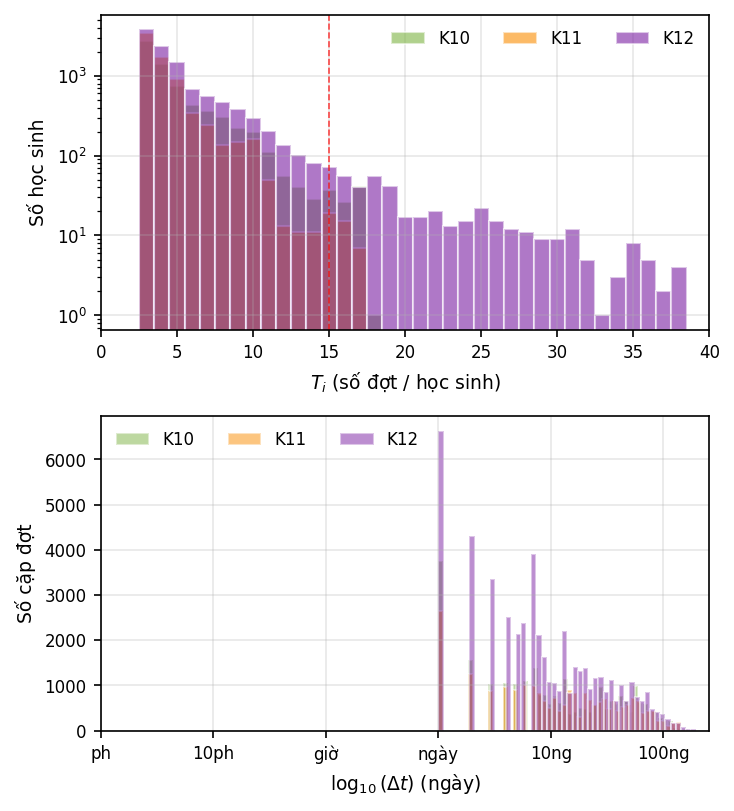
\includegraphics[width=\linewidth]{T_dt_distribution_vertical.png}
  \captionof{figure}{Phân phối $T_i$ (trên) và $\Delta t$ (dưới) theo khối. Đường đứt nét đỏ: ngưỡng $T_i \ge 15$ cho CT-DSEM.}
  \label{fig:Tdt}
\end{minipage}
\end{figure}

\subsubsection{Quy trình phân tích}

Quy trình phân tích gồm bảy bước nối tiếp (Hình~\ref{fig:pipeline}). Nhật ký làm bài trước hết được làm sạch và chuyển sang dạng dài, mỗi dòng là một đáp ứng của một học sinh với một câu hỏi trong một đợt (bước 1). Tính đơn chiều của ngân hàng câu hỏi được kiểm tra bằng phân tích nhân tố khám phá và biểu đồ giá trị riêng (bước 2) trước khi hiệu chuẩn độ khó \(b_j\) bằng mô hình 1PL, riêng cho từng khối (bước 3). Với các \(b_j\) đã cố định, năng lực của học sinh ở từng đợt được chấm bằng EAP, cho cặp \((\hat\theta_{it}, \seit)\) (bước 4). Chuỗi ước lượng này đi vào hai nhánh song song: các mô hình cấu trúc dọc phân tích quỹ đạo ở cấp khối (bước 5), còn bộ làm trơn Kalman hiệu chỉnh quỹ đạo của từng học sinh (bước 6). Kết quả của hai nhánh, cùng ngân hàng câu hỏi đã hiệu chuẩn, được dùng cho hai ứng dụng cảnh báo sớm và gợi ý câu hỏi (bước 7). Bước 1 được viết bằng Python; các bước còn lại dùng R với các gói \texttt{mirt}, \texttt{lavaan}, \texttt{lme4}, \texttt{ctsem} và \texttt{KFAS}.

\begin{figure}[H]
\centering
\resizebox{0.9\linewidth}{!}{%
\begin{tikzpicture}[
  font=\footnotesize,
  every node/.style = {align=center},
  box/.style   = {rectangle, draw, rounded corners=2pt, minimum width=24mm, minimum height=9mm, inner sep=2pt},
  arr/.style   = {-{Latex[length=1.6mm]}, thick},
  dasharr/.style = {-{Latex[length=1.6mm]}, thick, dashed, gray!70},
]
\node[box, fill=gray!12]   (s1) at (0,    0) {(1) Tiền xử lý\\ \scriptsize nhật ký $\to$ dạng dài};
\node[box, fill=blue!8]    (s2) at (3.5,  0) {(2) Kiểm tra đơn chiều\\ \scriptsize EFA, giá trị riêng};
\node[box, fill=blue!8]    (s3) at (7.0,  0) {(3) Hiệu chuẩn 1PL\\ \scriptsize độ khó $b_j$};
\node[box, fill=blue!8]    (s4) at (10.5, 0) {(4) Chấm điểm EAP\\ \scriptsize $\hat\theta_{it},\ \seit$};
\node[box, fill=orange!15] (s5) at (7.2, -1.8) {(5) Mô hình cấu trúc dọc\\ \scriptsize LGCM, LCSM, đa cấp, CT-DSEM};
\node[box, fill=green!15]  (s6) at (11.6,-1.8) {(6) Làm trơn Kalman\\ \scriptsize quỹ đạo từng học sinh};
\node[box, fill=red!12]    (s7) at (9.4, -3.4) {(7) Ứng dụng\\ \scriptsize cảnh báo sớm, gợi ý câu hỏi};
\draw[arr] (s1) -- (s2);
\draw[arr] (s2) -- (s3);
\draw[arr] (s3) -- (s4);
\draw[arr] (s4) -- (s5);
\draw[arr] (s4) -- (s6);
\draw[arr] (s5) -- (s7);
\draw[arr] (s6) -- (s7);
\draw[dasharr] (s3.south) to[bend right=30] (s7.west);
\end{tikzpicture}}
\caption{Quy trình phân tích bảy bước (mũi tên đứt nét: gợi ý câu hỏi dùng ngân hàng câu hỏi đã hiệu chuẩn ở bước 3).}
\label{fig:pipeline}
\end{figure}

% Tuyên bố Đạo đức và bảo mật dữ liệu đã được di chuyển xuống cuối bài
% (gộp cùng Lời cảm ơn + Mã nguồn) theo chuẩn paper quốc tế.
